\documentclass{jsarticle}

\usepackage{amsmath,amssymb}
\usepackage{bm}
\usepackage{braket}
\usepackage[dvipdfmx]{graphicx}
\usepackage{here}

\begin{document}
\part{ファンデル・ワールス-ロンドン相互作用の計算 補足}
	\section{初めに}
	原子半径に比べて大きな距離$R$だけ離れた2つの同じ希ガス原子を考えたとき、その2つの原子間にかかる相互作用を考える。詳しいことはキッテルの教科書p.57からp.61に書いてあるが、ここではp.60の式(4)と式(6)の導出を行う。

	\section{問題設定}
	一つのモデルとして、距離Rだけ離れた2つの同等な一次元調和振動子1と2を考える。各振動子はそれぞれに$x_{1}$と$x_{2}$だけ離れた電荷$\pm e$をもつ。運動量を$p_{1}$,$p_2$とする。以下に図を示す。\\
	\begin{figure}[H]
		\centering
		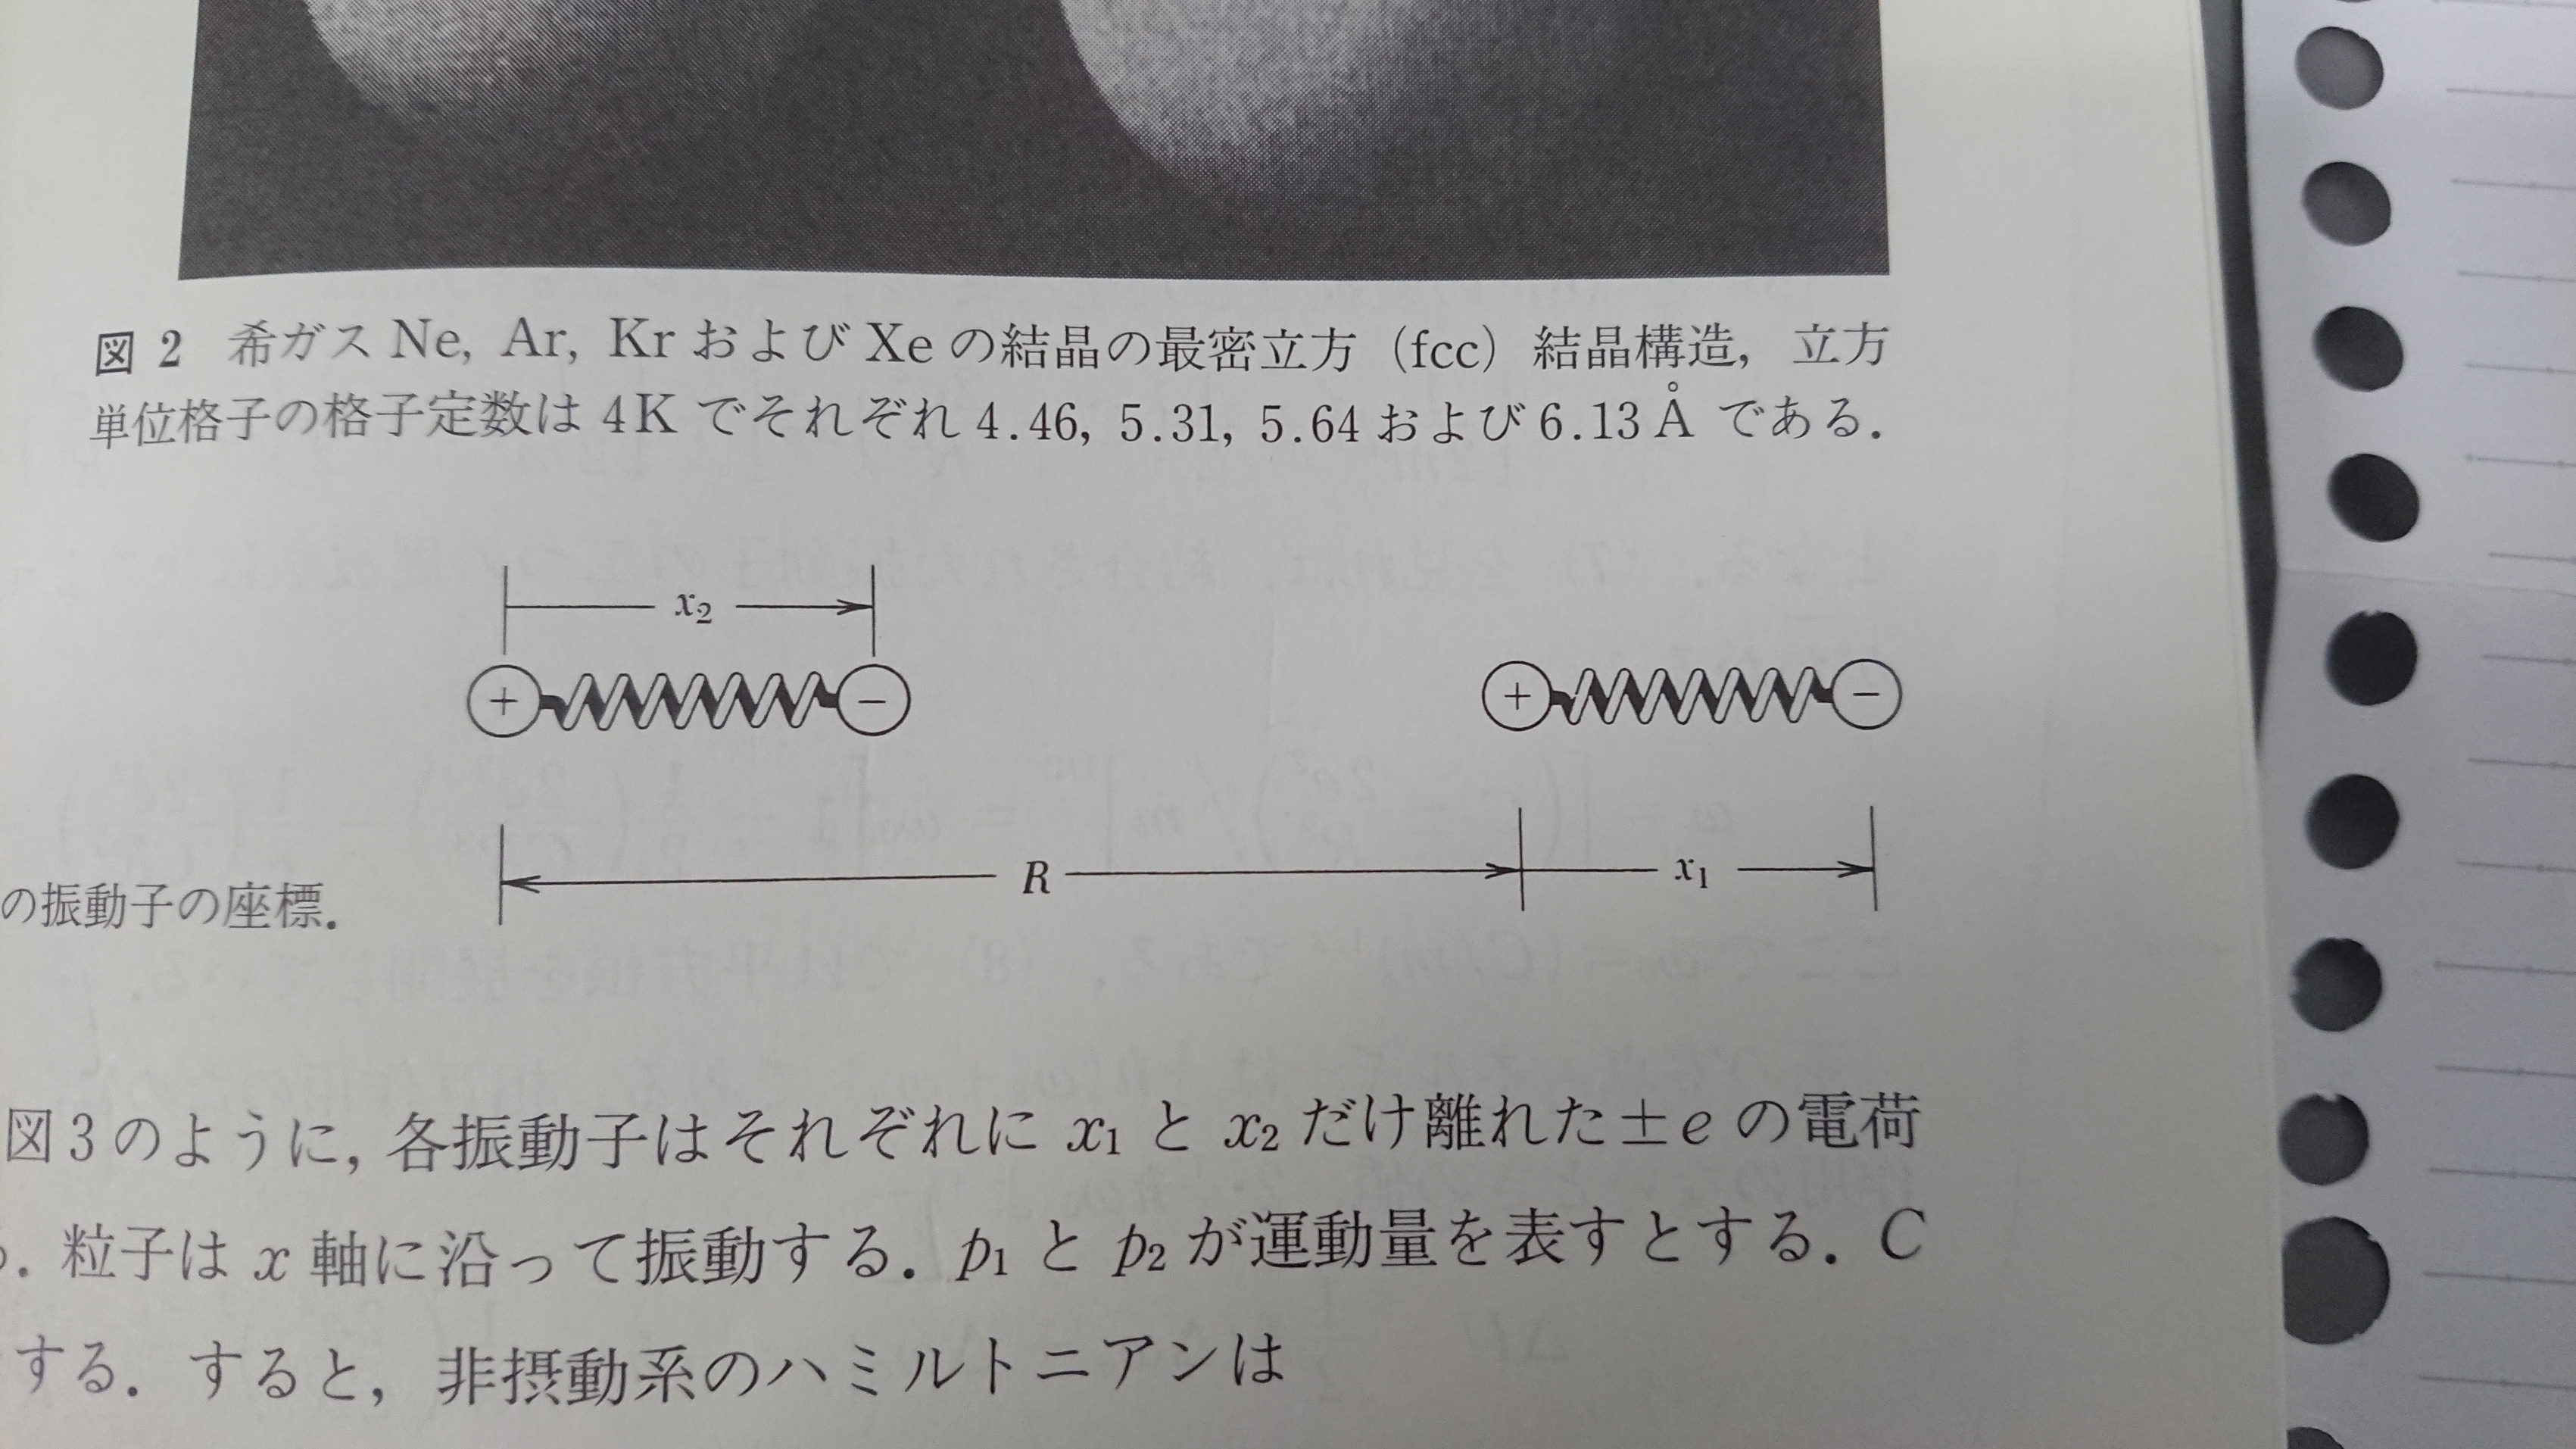
\includegraphics[width=0.7\linewidth]{DSC_0001}
		\caption{}
		\label{fig:dsc0001}
	\end{figure}

	このとき非摂動系のハミルトニアンは、力の定数Cとして、

		\begin{equation}
			H_{0}=\frac{1}{2m}p_{1}^{2}+\frac{1}{2}Cx_{2}^{2}+\frac{1}{2m}p_{2}^{2}+\frac{1}{2}Cx_{2}^{2}
		\end{equation}

	次に、2つの振動子のクーロン相互作用エネルギーを考える。このときのハミルトニアンをCGS系で考えると、

		\begin{equation}
			H_{1}=\frac{e^{2}}{R}+\frac{e^{2}}{R+x_{1}-x_{2}}-\frac{e^{2}}{R+x_{1}}-\frac{e^{2}}{R-x_{2}}
		\end{equation}

	$R$は十分大きいので、
		\begin{equation}
			H_{1}\tilde{=}-\frac{2e^{2}x_{1}x_{2}}{R^{3}}
		\end{equation}

	よって、全ハミルトニアンは、
		\begin{equation}
			H=H_{1}+H_{2}
		\end{equation}

	とおける。\\
	このとき、規準座標変換することで式(4)は完結な形に置き換えることができる。以降、変換後の座標$x_a$,$x_s$を求める。

	\section{計算過程}
	式(4)を行列を用いて表すと、
	\begin{equation}
		H=\frac{1}{2m}
		\begin{bmatrix}
		p_1 & p_2
		\end{bmatrix}
		\begin{bmatrix}
			1 & 0 \\
			0 & 1
		\end{bmatrix}
		\begin{bmatrix}
			p_1 \\
			p_2
		\end{bmatrix}
		+
		\begin{bmatrix}
		x_1 & x_2
		\end{bmatrix}
		\begin{bmatrix}
		\frac{C}{2} & -\frac{e^{2}}{R} \\
		-\frac{e^{2}}{R} & \frac{C}{2}
		\end{bmatrix}
		\begin{bmatrix}
		x_1 \\
		x_2
		\end{bmatrix}
	\end{equation}
	ここで、
	\begin{equation}
	\begin{bmatrix}
	\frac{C}{2} & -\frac{e^{2}}{R} \\
	-\frac{e^{2}}{R} & \frac{C}{2}
	\end{bmatrix}
	\end{equation}
	の固有値計算を行う。\\
	プログラムを用いて計算を行うと、
	\begin{equation}
	固有値 \lambda_1 = \frac{C}{2}+\frac{e^{2}}{R},
	固有ベクトル v_1=
	\begin{bmatrix}
	\frac{1}{\sqrt{2}} \\
	-\frac{1}{\sqrt{2}}
	\end{bmatrix}
	\end{equation}

	\begin{equation}
	固有値 \lambda_2 = \frac{C}{2}-\frac{e^{2}}{R},
	固有ベクトル v_2=
	\begin{bmatrix}
	\frac{1}{\sqrt{2}} \\
	\frac{1}{\sqrt{2}}
	\end{bmatrix}
	\end{equation}
	がわかる。\\
	ここから、
	\begin{equation}
	\begin{bmatrix}
	x_1 \\
	x_2
	\end{bmatrix}
	=
	\frac{1}{\sqrt{2}}
	\begin{bmatrix}
	1 & 1 \\
	1 & -1
	\end{bmatrix}
	\begin{bmatrix}
	x_s \\
	x_a
	\end{bmatrix}
	\end{equation}

	\begin{equation}
	\begin{bmatrix}
	p_1 \\
	p_2
	\end{bmatrix}
	=
	\frac{1}{\sqrt{2}}
	\begin{bmatrix}
	1 & 1 \\
	1 & -1
	\end{bmatrix}
	\begin{bmatrix}
	p_s \\
	p_a
	\end{bmatrix}
	\end{equation}
	とおくと、式(4)は、

	\begin{equation}
		H=\frac{1}{2m}p_s^2+\frac{1}{2}\left( C-\frac{2e^2}{R^3}\right) x_s^2+
		\frac{1}{2m}p_a^2+\frac{1}{2}\left( C+\frac{2e^2}{R^3}\right) x_s^2
	\end{equation}

	と置き換えることができる。\\
	Q.E.D
\end{document}
